% Created 2024-04-22 Mon 22:54
% Intended LaTeX compiler: pdflatex
\documentclass[11pt]{article}
\usepackage[utf8]{inputenc}
\usepackage[T1]{fontenc}
\usepackage{graphicx}
\usepackage{longtable}
\usepackage{wrapfig}
\usepackage{rotating}
\usepackage[normalem]{ulem}
\usepackage{amsmath}
\usepackage{amssymb}
\usepackage{capt-of}
\usepackage{hyperref}
\author{Rudolf Jovero}
\date{\today}
\title{musical pitch}
\hypersetup{
 pdfauthor={Rudolf Jovero},
 pdftitle={musical pitch},
 pdfkeywords={},
 pdfsubject={},
 pdfcreator={Emacs 29.2 (Org mode 9.7)}, 
 pdflang={English}}
\usepackage{calc}
\newlength{\cslhangindent}
\setlength{\cslhangindent}{1.5em}
\newlength{\csllabelsep}
\setlength{\csllabelsep}{0.6em}
\newlength{\csllabelwidth}
\setlength{\csllabelwidth}{0.45em * 3}
\newenvironment{cslbibliography}[2] % 1st arg. is hanging-indent, 2nd entry spacing.
 {% By default, paragraphs are not indented.
  \setlength{\parindent}{0pt}
  % Hanging indent is turned on when first argument is 1.
  \ifodd #1
  \let\oldpar\par
  \def\par{\hangindent=\cslhangindent\oldpar}
  \fi
  % Set entry spacing based on the second argument.
  \setlength{\parskip}{\parskip +  #2\baselineskip}
 }%
 {}
\newcommand{\cslblock}[1]{#1\hfill\break}
\newcommand{\cslleftmargin}[1]{\parbox[t]{\csllabelsep + \csllabelwidth}{#1}}
\newcommand{\cslrightinline}[1]
  {\parbox[t]{\linewidth - \csllabelsep - \csllabelwidth}{#1}\break}
\newcommand{\cslindent}[1]{\hspace{\cslhangindent}#1}
\newcommand{\cslbibitem}[2]
  {\leavevmode\vadjust pre{\hypertarget{citeproc_bib_item_#1}{}}#2}
\makeatletter
\newcommand{\cslcitation}[2]
 {\protect\hyper@linkstart{cite}{citeproc_bib_item_#1}#2\hyper@linkend}
\makeatother\begin{document}

\maketitle
\tableofcontents

Pitch is the perception of primarily frequency.
Frequency of sound waves is the sensation detected while musical pitch is the perception experienced.
\section{Elements of pitch}
\label{sec:org4e14d0b}
\subsection{Frequency}
\label{sec:org8a26f61}
The amount of cycles per second in a graphical representation of a wave.
While this is the primary determinant of pitch it is not the only determinant of pitch.
\subsection{Loudness}
\label{sec:orgf1561ef}

\begin{center}
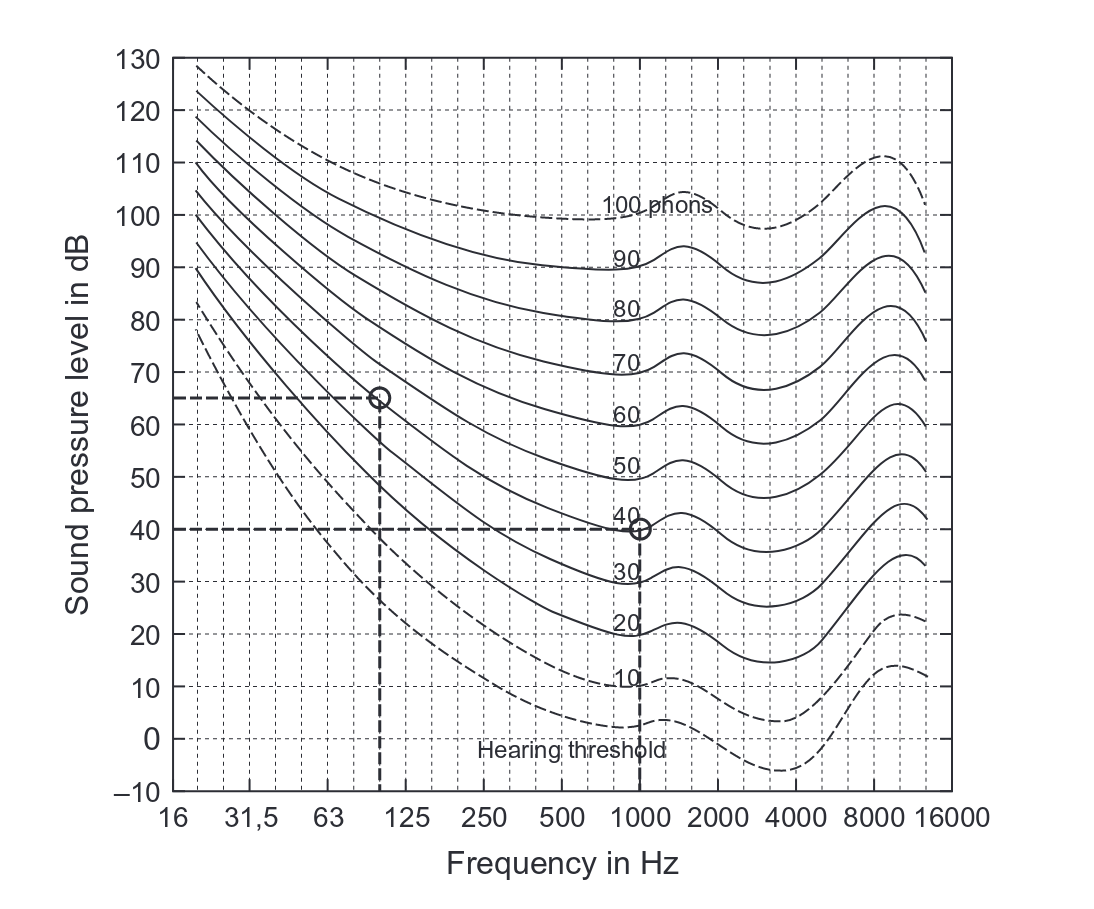
\includegraphics[width=.9\linewidth]{./images/Figure2PM.png}
\end{center}
\href{zotero://open-pdf/library/items/Z85TUTEI?page=5\&annotation=TG3KLECT}{pdf}
\href{zotero://select/library/items/ISHR544U}{“The Psychology Of Music”, 2013, p. 5}
\textbf{\textbf{Figure 2}} The equal-loudness contours, taken from ISO 226:2003.
Original figure kindly provided by Brian C. J. Moore. \cslcitation{1}{p. 5}



\begin{itemize}
\item Note taken on \textit{{[}2024-04-17 Wed 17:49] } \\
ISO 266:2003 has been withdrawn.
ISO 266:2023 is the current standard.
\end{itemize}
\subsubsection{Amplitude}
\label{sec:org01305b4}
The height from the equilibrium point in a wave.
Amplitude contributes to our perception of loudness.
Loudness in turn contributes to our perception of pitch.
However amplitude is not the whole story.
\section{Illusions of pitch}
\label{sec:orga571479}

\subsection{Shepard Tones}
\label{sec:orgc740baf}
Pitch chroma without definite pitch height.
\section{Relationships to other musical parameters}
\label{sec:org9fccce2}
\subsection{Rhythm}
\label{sec:org0b8fc2d}
\subsection{Tuning and Scales}
\label{sec:org4b830bb}
\subsection{Timbre and Spectrum}
\label{sec:org361d0fc}
\section{Bibliography}
\label{sec:org912de98}
\begin{cslbibliography}{0}{0}
\cslbibitem{1}{\cslleftmargin{[1]}\cslrightinline{D. Deutsch, Ed., \textit{The Psychology Of Music}, Third edition. Amsterdam: Academic Press, 2013. Available: \url{https://doi.org/10.1016/B978-0-12-381460-9.00001-8}}}

\end{cslbibliography}
\end{document}
